\chapter{Lecture}\label{part2:lec11} %% 11
\markboth{\thechapter. Lecture}{\thechapter. Lecture}

We\pageoriginale found that $\mathscr{V}_\alpha (\mathscr{V}, q)$ changes at most
its sign when $\mathscr{V}$ is replaced by $\mathscr{V}+1$, while it
picks up a trivial factor $A$ when $\mathscr{V}$ is replaced by
$\mathscr{V}+ \tau$. If we form quotients, $A$ will cancel out and we
may therefore expect to get doubly-periodic functions. Let us form
some useful quotients:
\begin{align*}
  f_2 (\mathscr{V}) & = \frac{\mathscr{V}_2(\mathscr{V},
    q)}{\mathscr{V}_1 (\mathscr{V}, q)}\\
  f_3 (\mathscr{V}) & = \frac{\mathscr{V}_3 (\mathscr{V},
    q)}{\mathscr{V}_1 (\mathscr{V}, q)}\\
  f_4 (\mathscr{V}) & = \frac{\mathscr{V}_4(\mathscr{V},
    q)}{\mathscr{V}_1 (\mathscr{V}, q)}
\end{align*}

For simplicity of location of poles it is convenient to take
$\mathscr{V}_1$ in the denominator since it has a zero at the
origin. From the table of the $\mathscr{V}$-functions we find that
these functions are not quite doubly periodic:
\begin{alignat*}{4}
  f_2 (\mathscr{V}+1) & = f_2 (\mathscr{V}) & \qquad & f_3 (\mathscr{V}+1) 
  = - f_3 (\mathscr{V})\\
  f_2 (\mathscr{V}+\tau) & = -f_2 (\mathscr{V}) && f_3 (\mathscr{V}+\tau)
   = -f_3 (\mathscr{V})\\
   && f_4 (\mathscr{V}+1)  = -f_4 (\mathscr{V})\\
   && f_4 (\mathscr{V}+\tau)  = f_4 (\mathscr{V})~~\,
\end{alignat*}

So\pageoriginale the functions are not doubly periodic; they do not
return to themselves. And we cannot expect that either. For suppose
any of the functions $f$ were actually doubly periodic. We know that
each has a pole of the first order per parallelogram. Integrating
round the parallelogram with vertices at $\pm \frac{1+ \tau}{2}, \pm
\frac{1-\tau}{2}$ (so that the origin which is the pole is enclosed),
we have
$$
\int f(\mathscr{V}) d \mathscr{V} =0 
$$

\begin{figure}[H]
\centering{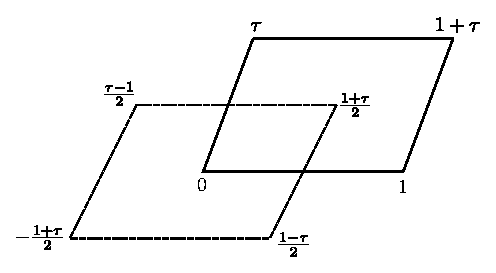
\includegraphics{vol2-figures/fig2.14.eps}}
\end{figure}
i.e., the sum of the residues at the poles =0. This means that either
the pole is a double is a double pole with zero residue, or there are
two simple poles with residues equal in magnitude but opposite in
sign. However neither of these is the case. So there is no necessity
for any further experimentation. 

Let us therefore consider the squares
$$
f^2_2 (\mathscr{V}), f_3^2 (\mathscr{V}), f_4^2 (\mathscr{V})
$$
these are indeed doubly periodic functions. And they are even
functions. So the expansion in the neighbourhood of the pole will not
contain the term of power $-1$. Hence the pole must be a double pole
with residue zero. So they are closely related to the Weierstrassian
function $\mathscr{P}(\mathscr{V})$, and must indeed be of the form $C
\mathscr{P}(\mathscr{V})+C_1$.

So\pageoriginale we have constructed doubly periodic functions. They
are essentially $\mathscr{P}(\mathscr{V})$. $\omega_1$ and $\omega_2$
of $\mathscr{P}(\mathscr{V})$ are our 1 and $\tau$. In order to get a
better insight we need the exact values of the functions. Let us
consider their pole terms. Expanding in the neighbourhood of the
origin,
\begin{align*}
  \frac{\mathscr{V}_\alpha (\mathscr{V}, q)}{\mathscr{V}_1
    (\mathscr{V}, q)} & = \frac{\mathscr{V}_\alpha +
    \frac{\mathscr{V}''_\alpha}{2!} \mathscr{V}^2 +
    \cdots}{\frac{\mathscr{V}'_1}{1!} \mathscr{V} +
    \frac{\mathscr{V}'''_1}{3!} \mathscr{V}^3 + \cdots}\\
  & = \frac{\mathscr{V}_\alpha}{\nu \mathscr{V}'_1}\left( \frac{1+
    \frac{1}{2} \frac{\mathscr{V}''_\alpha}{\mathscr{V}_\alpha} \nu^2
    + \cdots}{1+ \frac{\mathscr{V}'''_1}{6 \mathscr{V}'_1} \nu^2 +
    \cdots}\right)\\
  & = \frac{\mathscr{V}_\alpha}{\nu \mathscr{V}'_1} \left(1+
  \frac{1}{2}\frac{\mathscr{V}''_\alpha}{\mathscr{V}_\alpha} \nu^2 +
  \cdots \right) \left( 1- \left(\frac{\mathscr{V}'''_1}{6
    \mathscr{V}'_1} \nu^2 + \cdots\right)^2 + (\cdots)^3 -
  \cdots\right)\\
  & = \frac{\mathscr{V}_\alpha}{\nu\mathscr{V}'_1} \left(1+ \nu^2
  \left(\frac{\mathscr{V}''}{2\mathscr{V}_\alpha} -
  \frac{\mathscr{V}'''_1}{6 \mathscr{V}'_1} \right) + \cdots \right)\\
  \therefore \quad f_\alpha^2 & = \left( \frac{\mathscr{V}_\alpha
    (\mathscr{V}, q)}{\mathscr{V}_1 (\mathscr{V}, q)}\right)^2\\
  & = \frac{\mathscr{V}_\alpha^2}{\mathscr{V}{'2}_1}
  \frac{1}{\mathscr{V}^2} \left( 1+ \mathscr{V}^2
  \left(\frac{\mathscr{V}''_\alpha}{\mathscr{V}_1}-
  \frac{\mathscr{V}'''_1}{3 \mathscr{V}'_1} \right) + \cdots \right) 
\end{align*}

Let us now specialise $\alpha$. We have a special interest in
$\mathscr{V}_3$ because it is such a nice function: $\mathscr{V}_3 =
\sum\limits^\infty_{n=-\infty} q^{n^2}$. We have
$\dfrac{\mathscr{V}^{'2}_1}{\mathscr{V}^2_\alpha} f_\alpha^2
(\mathscr{V}) = \dfrac{1}{\mathscr{V}_2}+$ non-negative powers of
  $\mathscr{V}$. 

If\pageoriginale we take two such and take the difference, the difference will no
longer have a pole. Taking $\alpha=2, 4$, for instance,
\begin{equation*}
  \frac{\mathscr{V}^{'2}_1}{\mathscr{V}^2_2} \left(
  \frac{\mathscr{V}_2(\mathscr{V}, q)}{\mathscr{V}_1(\mathscr{V},
    q)}\right)^2 - \frac{\mathscr{V}^{'2}_1}{\mathscr{V}^2_4}
    \left(\frac{\mathscr{V}_4 (\mathscr{V},
      q)}{\mathscr{V}_1(\mathscr{V}, q)} \right)^2=
    \frac{\mathscr{V}''_2}{\mathscr{V}_2} -
    \frac{\mathscr{V}_4}{\mathscr{V}''_4}+\text{positive powers
      of}~\mathscr{V} \tag{*}\label{part2:lec11:eq*}
\end{equation*}

The left side is a doubly periodic function without a pole and so a
constant $C$; the right side is therefore just
$\dfrac{\mathscr{V}''_2}{\mathscr{V}_2}-
\dfrac{\mathscr{V}_4''}{\mathscr{V}_4}$. The vanishing of the other
terms on the other terms on the right side, of course, implies lots of
identities. 

So we have already computed $C$ in one way:
$$
C=\dfrac{\mathscr{V}''_2}{\mathscr{V}_2}-
\dfrac{\mathscr{V}_4''}{\mathscr{V}_4}
$$
 
To evaluate $C$ in other ways we may take in (\ref{part2:lec11:eq*})
$\mathscr{V}=\dfrac{1}{2}$, $\mathscr{V}=\dfrac{\tau}{2}$ or
$\mathscr{V}=(1+ \tau)/2$. From the table,
\begin{alignat*}{4}
  \mathscr{V}_1 \left(\frac{1}{2}, q\right) & = \mathscr{V}_2 &\qquad &
  \mathscr{V}_1 \left( \frac{1+\tau}{2} , q\right) = q^{-1/4}
  \mathscr{V}_3 \\
  \mathscr{V}_2 \left(\frac{1}{2}, q\right) & = -\mathscr{V}_1=0 &&
  \mathscr{V}_2 \left( \frac{1+\tau}{2} , q\right) = -iq^{-1/4}
  \mathscr{V}_4 \\
  \mathscr{V}_4 \left(\frac{1}{2}, q\right) & = \mathscr{V}_3 &&
  \mathscr{V}_4 \left( \frac{1+\tau}{2} , q\right) = q^{-1/4}
  \mathscr{V}_2 
\end{alignat*}

So\pageoriginale again from the left side of (\ref{part2:lec11:eq*}),
\begin{align*}
  C & = \frac{\mathscr{V}_1^{'2}}{\mathscr{V}_2^2} \times 0 -
  \frac{\mathscr{V}_1^2}{\mathscr{V}_4^2}
  \frac{\mathscr{V}_3^2}{\mathscr{V}_2^2}\\ 
  & = - \frac{\pi^2 \mathscr{V}_1^2
    \mathscr{V}_3^4}{\pi^2\mathscr{V}_2^2\mathscr{V}_3^2
    \mathscr{V}_4^2} =- \pi^2 \mathscr{V}_3^4
\end{align*}

Also
\begin{align*}
  C &= \frac{\mathscr{V}_1^{'2}}{\mathscr{V}_2^2} 
  \left( -\frac{\mathscr{V}_4^2}{\mathscr{V}_3^2}\right)-
  \frac{\mathscr{V}_1^{'2}}{\mathscr{V}_4^2}
  \frac{\mathscr{V}_2^2}{\mathscr{V}_3^2}\\
  & = -\frac{\pi^2\mathscr{V}_1^{'2}\mathscr{V}_4^4}
       {\pi^2\mathscr{V}_2^2\mathscr{V}_3^2\mathscr{V}_4^2} - 
       \frac{\pi^2\mathscr{V}_1^{'2}\mathscr{V}_2^4}
       {\pi^2\mathscr{V}_2^{2}\mathscr{V}_3^2\mathscr{V}_4^2}\\
  & = - \pi^2 \mathscr{V}^4_4 - \pi^2 \mathscr{V}_2^4
\end{align*}

From these we get an identity which is particularly striking:
\begin{equation*}
  \mathscr{V}_3^4 = \mathscr{V}_2^4 + \mathscr{V}_4^4
  \tag{1}\label{part2:lec11:eq1} 
\end{equation*}

We have also
\begin{equation*}
  \pi^2 \mathscr{V}_3^4 = \frac{\mathscr{V}_4''}{\mathscr{V}_4} -
  \frac{\mathscr{V}_2''}{\mathscr{V}_2}\tag{2}\label{part2:lec11:eq2} 
\end{equation*}

Now let us look at (\ref{part2:lec11:eq1}) and do a little
computing. Explicitly (\ref{part2:lec11:eq1}) 
states:
\begin{equation*}
  \left( \sum^\infty_{n=-\infty} q^{n^2}\right)^4 = \left( q^{1/4}
  \sum^\infty_{n=-\infty}q^{n(n+1)}\right)^4 + \left(
  \sum^\infty_{n=-\infty} (-)^n q^{n^2}\right)^4 \tag{3}\label{part2:lec11:eq3} 
\end{equation*}

This is an identity of some interest.

Let\pageoriginale us look for $q^N$ on both sides. The left side
gives $N$ in the form $N= n^2+n^2_2 + n_3^2 + n_4^2$, that is, as the
sum of four squares. So dies the second term on the right. If $N$ is
even, it is trivial that both sides are in agreement because the first
term on the right gives only odd powers of $q$, and the coefficient of
$q^n$ in the second term on the right is
$$
\sum_{n_1^2 n_2^2+ n_3^2 +n_4^2=N} (-)^{n_1+n_2+n_3+n_4}
$$ 

Since $N$ is even either all $n_i$'s are odd, or two of them odd,
or none. It is not transparent. What happens when $N$ is odd. 

Take the more interesting formula (\ref{part2:lec11:eq2}):
$$
\pi \mathscr{V}^4_3 = \frac{\mathscr{V}_4''}{\mathscr{V}_4} -
\frac{\mathscr{V}_2''}{\mathscr{V}_2} 
$$

By the differential equation,
\begin{align*}
  \mathscr{V}_\alpha'' & = \left[ \frac{\partial^2}{\partial
      \mathscr{V}^2} \mathscr{V}_\alpha (\mathscr{V},
    q)\right]_{\mathscr{V}=0}\\
  & = \left[ - 4 \pi^2 q \frac{\partial}{\partial q}
    \mathscr{V}_\alpha (\mathscr{V}, q)\right]_{\mathscr{V}=0}\\
  \therefore \quad \mathscr{V}_3^4 & = 4 q
  \left(\frac{1}{\mathscr{V}_2} \frac{\partial \mathscr{V}_2}{\partial
    q} - \frac{1}{\mathscr{V}_4} \frac{\partial
    \mathscr{V}_4}{\partial q} \right)\\
  & = 4q \frac{\partial}{\partial q} \log
  \frac{\mathscr{V}_2}{\mathscr{V}_4} 
\end{align*}

Now\pageoriginale 
\begin{align*}
  \frac{\mathscr{V}_2}{\mathscr{V}_4} & = 2 q^{1/4}
  \frac{\prod\limits^\infty_{n=1} (1- q^{2n}) (1+
    q^{2n})^2}{\prod\limits^\infty_{n=1}(1-q^{2n})(1-q^{2n-1})}\\
  &= 2 q^{1/4}  \frac{\prod\limits^\infty_{n=1} (1- q^{2n})^2 (1+
    q^{2n})^2}{\prod\limits^\infty_{n=1}(1-q^{2n})^2 (1-q^{2n-1})^2}\\
  & =2 q^{1/4} \frac{\prod\limits^\infty_{n=1} (1- q^{4n})^2}
       {\prod\limits^\infty_{n=1}(1-q^{n})^2}\\
  & = \frac{2q^1/4}{\prod\limits_{4 ~\nmid~ n}(1-q^n)^2}     
\end{align*}

Taking the logarithmic derivative,
\begin{align*}
  \mathscr{V}_3^4 & = 4q \left\{ \frac{1}{4q} -2 \sum_{4 ~\nmid~
    n} \frac{-n q^{n-1}}{1- q^n}\right\}\\
  & = 1+ 8 \sum_{4 ~\nmid~ n} \frac{n q^n}{1-q^n}\\
  & = 1+ 8 \sum_{4 ~\nmid~ n} n\sum^\infty_{k=1} q^{nk}\\
  & = 1+ 8 \sum_{\substack{4 ~\nmid~ m\\m=1}} q^{m} \sum_{n|m}n\\
  & = 1+ 8 \sum^\infty_{m=1} \sigma^* (m) q^m
\end{align*}
with\pageoriginale the previous that $\displaystyle{\sigma^* (m) = \sum_{d/m},
\mathop{d}_{4 ~\nmid~\alpha}}$, that is the divisor sum with those\break
divisors omitted which are divisible by 4. This is an interesting identity:
\begin{equation*}
  \left( \sum^\infty_{n=-\infty} q^{n^2}\right)^4 = 1+8
  \sum^\infty_{m=1} \sigma^* (m) q^m \tag{4}\label{part2:lec11:eq4}
\end{equation*}

On the left $q^m$ can be obtained only as $q^{n_1^2+ n_2^2 + n_3^2+
  n_4^2}$, so that the coefficient of $q^m$ on the right is the number
of ways in which this representation for $m$ is possible; $m$ is as
often the sum of four squares as $8 \sigma^* (m)$. Clearly $\sigma^*
(m) \neq 0$, since among the admissible divisors, 1 is always
present. So $\sigma^* (m) \geq 1$, or every $m$ does admit at least
one such representation. We have thus proved \textit{Lagrange's
  theorem}: Every integer is the sum of at most four squares. 

If $m$ is odd, $\sigma^* (m) = \sigma (m)$; if $m$ is even, 
\begin{align*}
  \sigma^* (m) & = \sum_{d|m, ~d~\text{odd}} d + 2 \sum_{d|m,~
    d~\text{odd}}d\\
  & = 3 \sum_{d|m, ~d~\text{odd}} d
\end{align*}

If we denote by $r_4(m)$ the number of representations of $m$ as the
sum of four squares, then 

\begin{tabbing}
  $r_4(m)$ \= = 8 times the sum of odd divisors of $m$, $m$ odd;\\
  \> \quad 24 times the sum of odd divisors of $m$, $m$ even.
\end{tabbing}

We have not partitions this time, but representation as the sum of
squares. We agree to consider as distinct these representations in
which the order of the components has been changed. In partitions
we\pageoriginale abstracted from the order of the summands; here we
pay attention to order, and also to the sign (i.e., one representation
$n_1^2 + n_2^2 + n_3^2 +n_4^2$ is actually counted, order apart, as 16
different representations $(\pm n_1)^2 + (\pm n_2)^2 +(\pm n_3)^2+(\pm
n_4)^2$, if $n_1, n_2, n_3, n_4$ are all different from 0).

As an example, take $m=10$. The different representations as the sum
of four squares are 
\begin{gather*}
  (\pm 1)^2 + (\pm 1)^2 + (\pm 2)^2 + (\pm 2)^2,\\
  (\pm 1)^2+ (\pm 3)^2+ (0)^2+ (0)^2,
\end{gather*}
along with their rearrangements, six in each. Thus altogether
\begin{align*}
  r_4 (10) & = 6 \times 16 + 6\times 8 = 144\\
  8 \sigma^* (10) & = 3(1+2+5+10) = 8 \times 18 = 144
\end{align*}

Lagrange's theorem was first enunciated by Fermat in the seventeenth
century. Many mathematicians tried to solve it without success;
eventually Jacobi found out the identity
$$
r_4 (m) = 8 \sigma^* (m)
$$

Before that, the fact that every integer is the sum of four squares
was conjectured by Fermat, Euler did not succeed in proving it. It was
proved by Lagrange, and later Euler gave a mere elementary
proof. Euler proved that if two numbers are each the sum of four
squares, then so is their product, by means of the identity:
\begin{multline*}
  (x_1^2 + x_2^2 + x_3^2 + x_4^2)(y_1^2 + y_2^2 + y_3^2+ y_4^2)\\
  = (x_1 y_1+ x_2y_2+ x_3 y_3 + x_4 y_4)^2 + (x_1 y_2- x_2y_1 + x_3
  y_4 - x_4 y_3)^2 +\\
  + (x_1y_3 - x_3 y_1 + x_4y_2 - x_2 y_4)^2 + (x_1y_4- x_4 y_1 + x_2
  y_3 - x_3 y_2)^2.
\end{multline*}

We\pageoriginale do not proceed to discuss in detail the representability of a
number as the sum of two sequences.

If we return not to $f_\alpha^2$ but to $f_\alpha$ we are not helpless
to deal with them. $f_4$ is not doubly periodic in the fundamental
parallelogram, but is doubly periodic in a parallelogram of twice this
size with vertices at $0, 2, 2+ \tau, \tau$. It has got a pole at the
vertex 0 and another at the vertex 1, with residues adding up to
zero. 
\begin{figure}[H]
  \centering{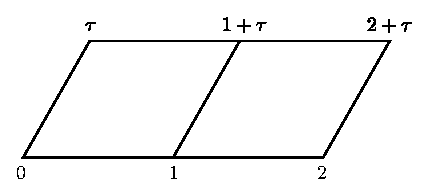
\includegraphics{vol2-figures/fig2.15.eps}}
\end{figure}

We may write down another identity:
$$
\frac{\mathscr{V}_1'}{\mathscr{V}_4} \cdot
\frac{\mathscr{V}_4(\mathscr{V}/\tau)}{\mathscr{V}_1
  (\mathscr{V}/\tau)}
= \frac{1}{2} \left\{ \frac{\mathscr{V}_1' \left(
  \frac{\mathscr{V}}{2}\Big/
  \frac{\tau}{2}\right)}{\mathscr{V}_1\left( \frac{\mathscr{V}}{2}
  \Big/ \frac{\tau}{2}\right)} - \frac{\mathscr{V}_1'\left(
  \frac{\mathscr{V}+1}{2} \Big/ \frac{\tau}{2}\right)}{\mathscr{V}_1
  \left( \frac{\mathscr{V}+1}{2} \Big/ \frac{\tau}{2}\right)}\right\} 
$$

This may be deduced by checking that the poles on both sides are the
same, Further they are odd functions and so the constant term in the
difference must vanish. Put $\mathscr{V}= \dfrac{1}{2}$ on both
sides. 

Then\pageoriginale we get
$$
\pi \mathscr{V}_3^2
= \frac{1}{2} \left\{ \frac{\mathscr{V}_1' \left(
  \frac{1}{4}\Big/ \frac{\tau}{2}\right)}{\mathscr{V}_1\left( \frac{1}{4}
  \Big/ \frac{\tau}{2}\right)} - \frac{\mathscr{V}_1'\left(
  \frac{3}{4} \Big/ \frac{\tau}{2}\right)}{\mathscr{V}_1
  \left( \frac{3}{4} \Big/ \frac{\tau}{2}\right)}\right\} 
$$

By straightforward calculation, taking logarithmic derivatives, we
obtain, 
$$
\mathscr{V}_3^2 = 4 \sum^\infty_{m=1} q^m (\sigma_\circ^{(1)} (m) -
\sigma_\circ^{(3)} (m)),
$$
where the notation employed is:
\begin{align*}
  \sigma_k(m) & = \sum_{d|m} d^k,\\
  \sigma_\circ (m) & = \sum_{d|m} d^\circ = \text{number of divisors
    of}~m;\\
  \sigma_\circ^{(j)} (m) & = \mathop{\sum ~d^\circ}_{d|m, ~d\equiv j \pmod{4}}
\end{align*}
comparing coefficients of $q^m$, and observing that on the left $m$
occurs only in the form $n_1^2 + n^2_2$, we get the beautiful theorem:
\begin{tabbing}
  \qquad \= $m$\quad  \= can be represented as the sum of two squares as
  often\\
  \> as \> $4(\sigma_\circ^{(1)} (m) - \sigma_\circ^{(3)} (m))$.
\end{tabbing}

Notice that $\sigma_\circ^{(1)}(m) - \sigma_\circ^{(3)}(m)$ is always
non negatives; hence $\sigma_\circ^{(1)}(m) \geq
\sigma_\circ^{(3)}(m)$ (i.e., the number of divisors of the form
$4r+1$ is never less than the number of divisors of the form
$4r+1$), which is by no means a trivial fact.

In\pageoriginale some cases we can actually find out what the
difference $\sigma_\circ^{(1)}(m)- \sigma_\circ^{(3)} (m)$ will
be. Suppose that $m$ is a prime $p$. Then the only divisors are 1 and
$p$. The divisor 1 goes into $\sigma_\circ^{(1)}$; and $p$ goes into
$\sigma_\circ^{(3)}$ if $p \equiv 3 \pmod{4}$. So the difference is
zero. However, if $p \equiv 1 \pmod{4}$. $p$ goes into
$\sigma_\circ^{(1)}$. Hence the number of representations of a prime $p
\equiv 1 \pmod{4}$ as the sum of two squares is $4 \times 2 =8$. That
the number of representations of a prime $p \equiv 1 \pmod{4}$ as the
sum of two squares is 8 is a famous theorem of Fermat, proved for the
first time by Euler. It is usually proved by using the Gaussian
complex numbers. 

So far we have been looking upon $\mathscr{V}$ as the variable in the
$\mathscr{V}$- functions; now we proceed to consider $q$ as the
variable and go to deeper things like the Jacobi transformation.

